%==============================================================================
% Sjabloon poster bachproef
%==============================================================================
% Gebaseerd op document class `a0poster' door Gerlinde Kettl en Matthias Weiser
% Aangepast voor gebruik aan HOGENT door Jens Buysse en Bert Van Vreckem

\documentclass[a0,portrait]{hogent-poster}

% Info over de opleiding
\course{Graduaatsproef}
\studyprogramme{Graduaat in het Programmeren}
\academicyear{2024-2025}
\institution{Hogeschool Gent, Valentin Vaerwyckweg 1, 9000 Gent}

% Info over de bachelorproef
\title{Back-end Spring Boot: D\&D Character Generator}
\author{Thomas Gielen}
\email{thomas.gielen@student.hogent.be}
\supervisor{Luc Vervoort}
\cosupervisor{David Breckx}

% Indien ingevuld, wordt deze informatie toegevoegd aan het einde van de
% abstract. Zet in commentaar als je dit niet wilt.
\specialisation{Programmeren}
\keywords{Back-end, Spring Boot, Java}
\projectrepo{https://github.com/GielenThomas/Graduaatsproef}

\begin{document}

\maketitle

\begin{abstract}
Deze graduaatsproef beschrijft de ontwikkeling van een RESTful API in Spring Boot voor het aanmaken en beheren van Dungeons \& Dragons-personages. De API werd ontworpen volgens de documentation-first methode met Apidog en ondersteunt spelregels zoals klassen, rassen en statistieken. Het project toont aan hoe moderne backendtechnologie ingezet kan worden om spelers digitaal te ondersteunen.
\end{abstract}

\begin{multicols}{2} % This is how many columns your poster will be broken into, a portrait poster is generally split into 2 columns

\section{Introductie}

Dungeons \& Dragons is een rollenspel waarbij spelers complexe personages beheren. Dit gebeurt vaak handmatig of met beperkte digitale tools. Deze graduaatsproef onderzoekt hoe een Spring Boot API het aanmaken en beheren van deze personages kan vereenvoudigen.
De API is ontwikkeld met een documentation-first aanpak via Apidog en ondersteunt elementen zoals rassen, klassen en statistieken. Het project toont hoe moderne backendtechnologie kan worden ingezet om spelers en ontwikkelaars digitaal te ondersteunen.



\section{Wat heb ik bijgeleerd?}

Tijdens deze graduaatsproef werd veel bijgeleerd over de werking en structuur van het Java-framework Spring Boot, dat voordien onbekend was. Er werd inzicht verworven in hoe RESTful API's opgebouwd worden, inclusief routing, controllers en databindings.
Daarnaast werd kennis opgedaan over het OpenAPI-specificatieformaat en hoe een documentation-first aanpak met Apidog kan bijdragen aan duidelijke en consistente API-documentatie.

\section{Screenshot}



\begin{center}
  \captionsetup{type=figure}
  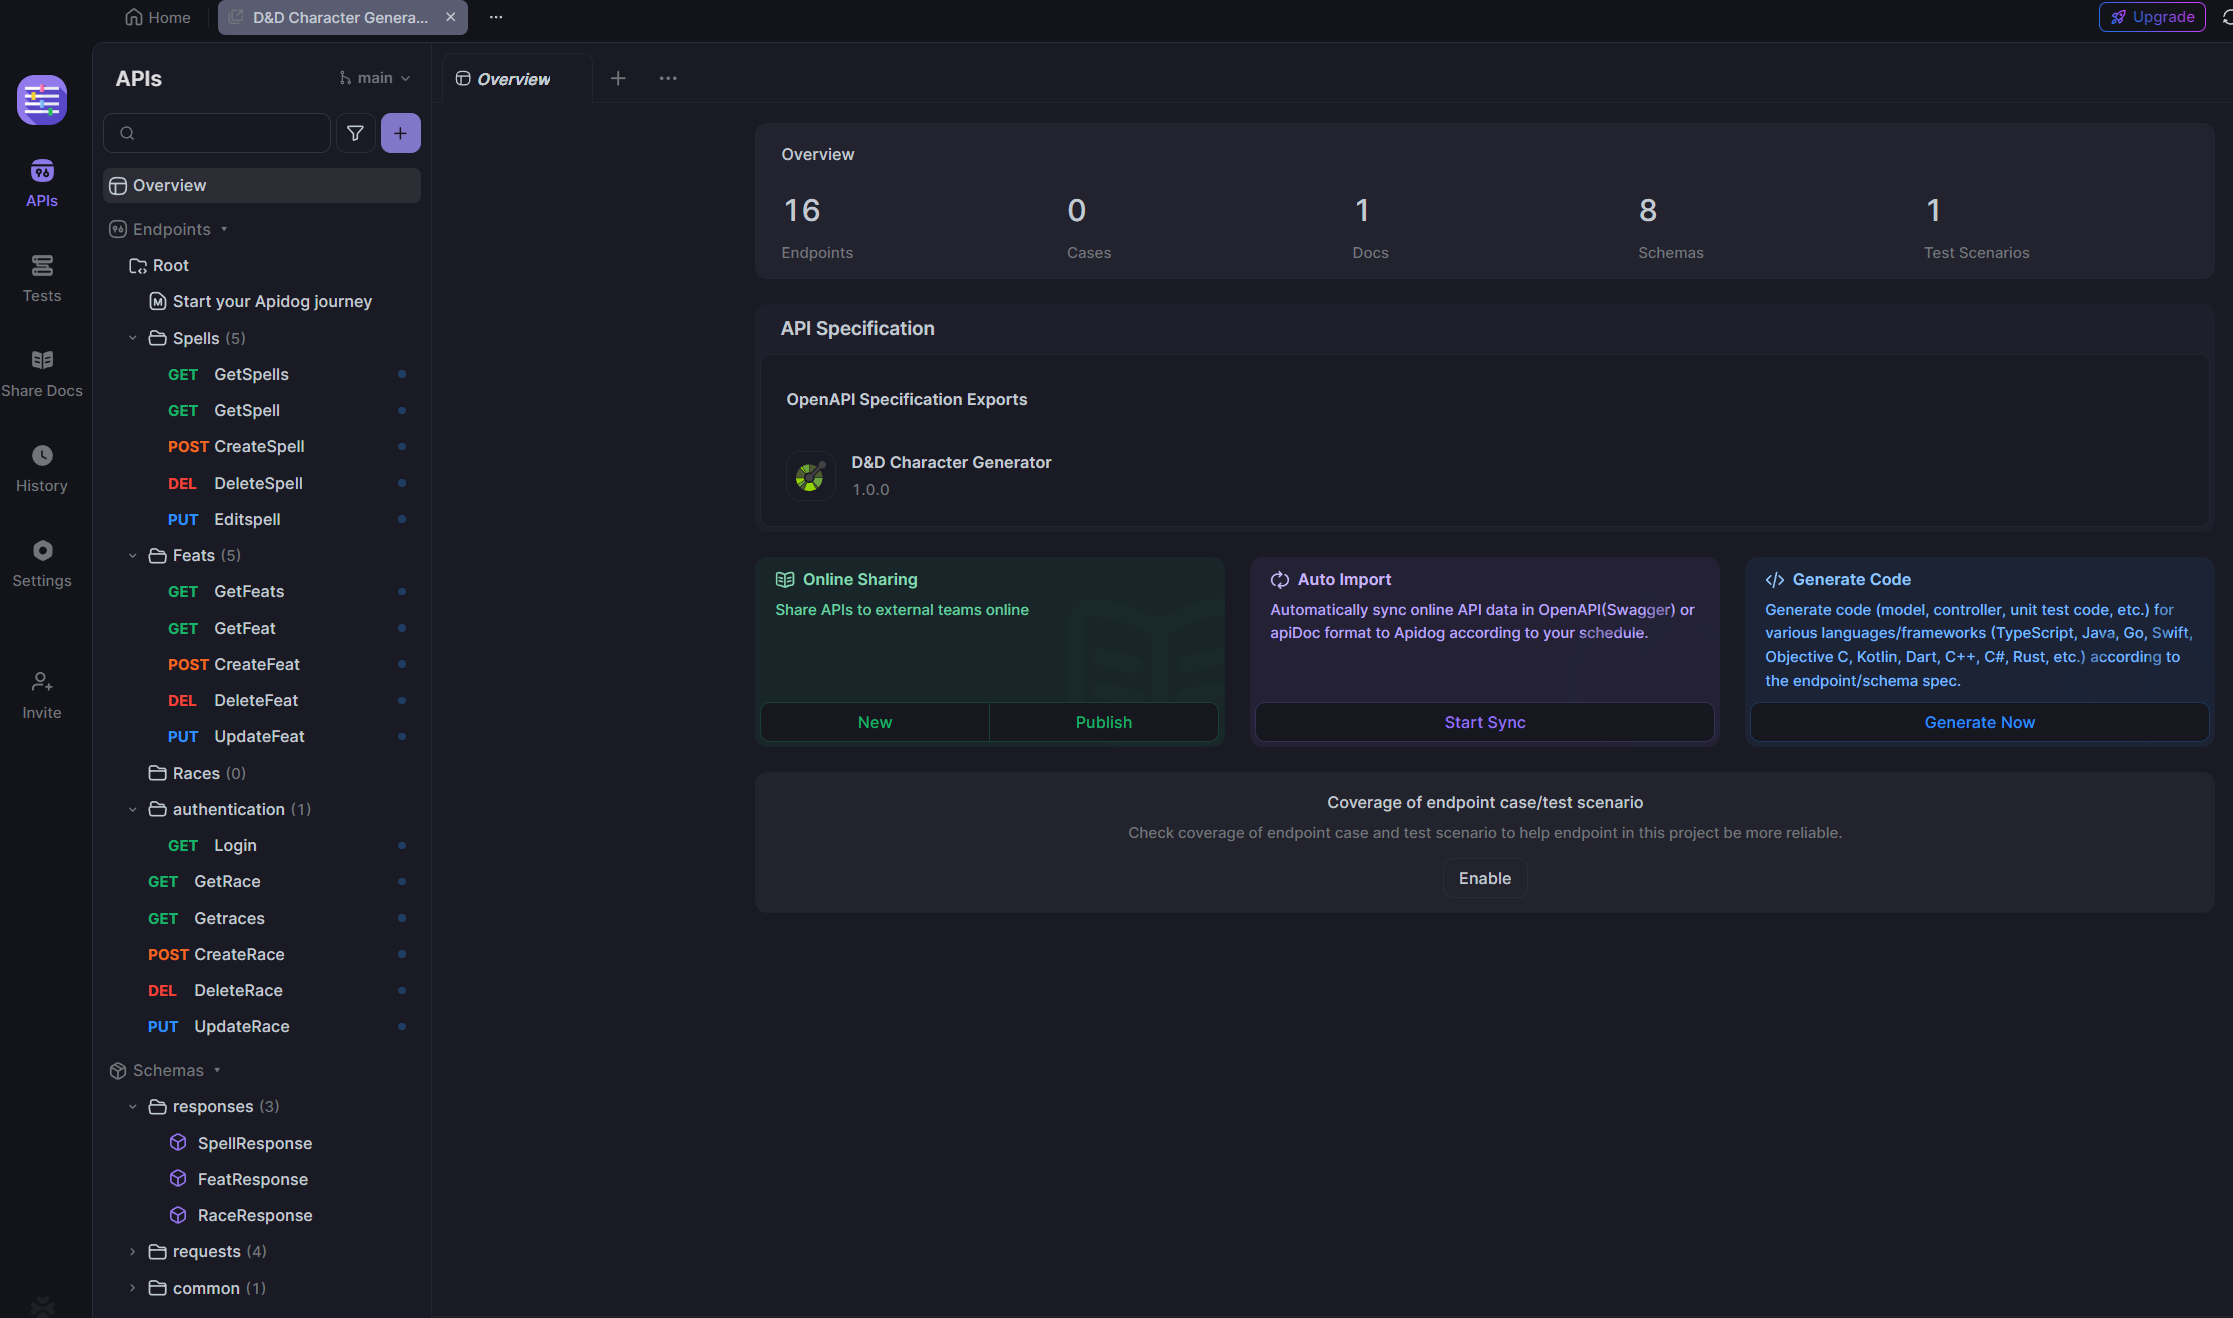
\includegraphics[width=1.0\linewidth]{Poster.png}
  \captionof{figure}{Screenshot van het Apidog project}
\end{center}

\section{Conclusies}

Deze graduaatsproef toont aan dat een Spring Boot API een efficiënte en uitbreidbare oplossing biedt voor het digitaal beheren van Dungeons \& Dragons-personages. Dankzij de documentation-first aanpak met Apidog werd een gestructureerde ontwikkeling gerealiseerd, met duidelijke specificaties en goed gedocumenteerde endpoints.
Hoewel Spring Boot in het begin nieuw en complex was, bleek het een krachtig framework voor het bouwen van RESTful API's. Het eindresultaat is een functioneel prototype dat spelmechanismen zoals rassen, klassen en statistieken ondersteunt, en dat eenvoudig verder uitgebreid kan worden.
Dit project bevestigt dat moderne backendtechnologieën ook buiten klassieke bedrijfscontexten inzetbaar zijn — bijvoorbeeld in de spelwereld — en biedt een waardevolle basis voor toekomstige toepassingen of uitbreidingen.

\section{Toekomstig onderzoek}

Met een werkende API en ingebouwde gebruikersauthenticatie vormt dit project een solide basis voor verdere ontwikkeling. Een volgende stap kan het uitbreiden van de functionaliteit zijn, zoals ondersteuning voor spelregels van andere Dungeons \& Dragons-edities of andere tabletop RPG-systemen.
Daarnaast kan onderzocht worden hoe de API gekoppeld kan worden aan een frontendtoepassing, zodat gebruikers via een gebruiksvriendelijke interface personages kunnen aanmaken en beheren. Ook schaalbaarheid en performantie bij intensiever gebruik zijn relevante onderzoekspunten, vooral als de API geïntegreerd wordt in grotere spelplatformen.
Tot slot kan het interessant zijn om een persistentielaag met geavanceerdere datamodellen toe te voegen, bijvoorbeeld met ondersteuning voor sessies, inventaris of spelvoortgang.

\end{multicols}
\end{document}